% RNGD AI Studio -- final presentation (compile: tectonic RNGD_final_presentation.tex)
\documentclass[9pt,aspectratio=169]{beamer}
\usetheme{metropolis}
\usepackage{graphicx}
\usepackage{xcolor}
\usepackage{booktabs}
\usepackage{tikz}
\usetikzlibrary{arrows.meta,positioning}

\definecolor{blueprint}{HTML}{1E5AA8}
\definecolor{blueprintdeep}{HTML}{123A6E}
\definecolor{amber}{HTML}{C98A12}
\definecolor{paper}{HTML}{F5F1E7}
\definecolor{ink}{HTML}{182228}
\definecolor{muted}{HTML}{5B6670}
\definecolor{critical}{HTML}{A32A21}
\definecolor{ok}{HTML}{2E6B47}

\setbeamercolor{frametitle}{bg=blueprintdeep,fg=paper}
\setbeamercolor{normal text}{bg=paper,fg=ink}
\setbeamercolor{background canvas}{bg=paper}
\setbeamercolor{progress bar}{fg=amber,bg=blueprint!20}
\setbeamercolor{alerted text}{fg=critical}
\setbeamercolor{block title}{bg=blueprint!14,fg=blueprintdeep}
\setbeamercolor{block body}{bg=blueprint!5,fg=ink}
\setbeamerfont{frametitle}{size=\Large}
\metroset{block=fill,progressbar=frametitle,numbering=fraction,sectionpage=none}
\graphicspath{{../walkthrough/screens/}{../walkthrough/optimizer/}{../optimization/}}
\setlength{\parskip}{0.3em}

\newcommand{\shot}[2]{\fcolorbox{blueprint!30}{white}{\includegraphics[width=\dimexpr#1-8pt\relax]{#2}}}
\newcommand{\shoth}[2]{\fcolorbox{blueprint!30}{white}{\includegraphics[height=#1]{#2}}}
\newcommand{\bignum}[2]{{\color{#1}\fontsize{30}{32}\selectfont\bfseries #2}}
\newcommand{\divider}[3]{{%
\setbeamertemplate{footline}{}
\begin{frame}[plain]
\begin{tikzpicture}[remember picture,overlay]
  \fill[blueprintdeep] (current page.south west) rectangle (current page.north east);
\end{tikzpicture}
\vspace*{2.2cm}
{\color{amber}\large\bfseries #1}\\[0.5cm]
{\color{paper}\Huge\bfseries #2}\\[0.5cm]
{\color{paper!75}\large #3}
\end{frame}}}

\begin{document}

% ------------------------------------------------------------------ title
{\setbeamertemplate{footline}{}
\begin{frame}[plain]
\begin{tikzpicture}[remember picture,overlay]
  \fill[blueprintdeep] (current page.south west) rectangle (current page.north east);
\end{tikzpicture}
\vspace*{0.9cm}
{\color{amber}\small\bfseries RNGD \ \textbullet\ CONCEPT-TO-SCHEMATIC AI STUDIO}\\[0.7cm]
{\color{paper}\fontsize{22}{27}\selectfont\bfseries A better way to lay out a hotel floor,\\[0.15cm] and the studio around it}\\[0.7cm]
{\color{paper!80}\large Layout optimization compared with the reference, then the whole system:\\ its parts, how they work, how they differ and what they achieved}\\[1.1cm]
{\color{paper!65}Naimul Haque \ \textbullet\ Semester project with RNGD \ \textbullet\ October 2026}
\end{frame}}

% ------------------------------------------------------------------ agenda
\begin{frame}{What I will show}
\begin{columns}[T]
\begin{column}{0.47\textwidth}
\begin{block}{Part 1 \ \textbullet\ Layout optimization}
\begin{itemize}
\item The job, and the reference optimizer
\item What was wrong with its floor plans
\item My updated optimizer, in plain terms
\item Side-by-side results on the same sites
\item Letting it choose the building shape too
\end{itemize}
\end{block}
\end{column}
\begin{column}{0.47\textwidth}
\begin{block}{Part 2 \ \textbullet\ The whole studio}
\begin{itemize}
\item How we use the BaaP idea
\item The five parts of the studio
\item How each part works, with screenshots
\item How the parts differ
\item Results, limits and next steps
\end{itemize}
\end{block}
\end{column}
\end{columns}
\end{frame}

\divider{PART 1}{Layout optimization}{The reference optimizer and my updated one, on the same sites}

% ------------------------------------------------------------------ the job
\begin{frame}{The job: fit a hotel's rooms onto a floor}
\begin{columns}[T]
\begin{column}{0.52\textwidth}
\textbf{What goes in}
\begin{itemize}
\item A floor outline on several levels, with the stairs and elevators marked
\item A list of rooms to place: here 72 rooms, 69 of them guest rooms
\end{itemize}
\textbf{What comes out}
\begin{itemize}
\item Where the corridor runs (the same on every level, so floors stack)
\item Where each room sits, with its door on the corridor
\end{itemize}
\textbf{What makes a plan good}
\begin{itemize}
\item As many rooms placed as possible
\item A window for every guest room
\item Little corridor, safe exits, accessible rooms
\end{itemize}
\end{column}
\begin{column}{0.44\textwidth}
\begin{block}{Why a computer should search}
There are far too many possible plans to try by hand. An optimizer tries hundreds of plans, scores each one, and keeps improving.
\end{block}
\begin{block}{Three test sites}
The prototype's three floor outlines (fp1, fp2, fp3), each with the same 72-room program.
\end{block}
\end{column}
\end{columns}
\end{frame}

% ------------------------------------------------------------------ reference
\begin{frame}{The starting point: the reference optimizer}
\begin{columns}[T]
\begin{column}{0.55\textwidth}
The prototype uses a \textbf{genetic algorithm} (Busra's work). In plain terms:
\begin{enumerate}
\item Start with many random plans.
\item Score them and keep the better ones.
\item Make new plans by \emph{mixing} two good plans and making small random changes.
\item Repeat, here for 500 rounds.
\end{enumerate}
In this version a plan is described by corridor pieces that can sit \textbf{anywhere} on the floor. Rooms are then attached wherever they touch a corridor.

{\small\color{muted} I had the result files for the three sites, not the source code. I rebuilt each delivered plan and scored it with the same scoring I use for my own.}
\end{column}
\begin{column}{0.4\textwidth}
\begin{block}{Reference results, three sites}
\centering
\bignum{blueprintdeep}{171 of 216}\\ rooms placed\\[0.5cm]
\bignum{critical}{24}\\ guest rooms without a window
\end{block}
\end{column}
\end{columns}
\end{frame}

% ------------------------------------------------------------------ problems
\begin{frame}{What I saw in its floor plans}
\begin{columns}[T]
\begin{column}{0.31\textwidth}
\begin{block}{Rooms without windows}
Nothing tells the search where the outside wall is, so whether a room gets a window is luck.
\end{block}
\begin{block}{Wasted floor area}
Rooms are dropped in one at a time. The gaps left over are odd shapes nobody can use.
\end{block}
\end{column}
\begin{column}{0.31\textwidth}
\begin{block}{Mixing plans rarely helps}
Half of one plan glued to half of another seldom makes a sensible building.
\end{block}
\begin{block}{Slow, and different every run}
My own first version also asked an AI model to judge plans during the search: about ten minutes, and never the same answer twice.
\end{block}
\end{column}
\begin{column}{0.31\textwidth}
\begin{block}{No idea of the limit}
It reports what it placed, but cannot say whether all the rooms could fit at all.
\end{block}
\begin{block}{Shape is fixed}
The building outline and the stair positions are given. It cannot try a different shape or more floors.
\end{block}
\end{column}
\end{columns}
\vspace{0.2cm}
{\small\color{muted} These points come from the reference results, from my first attempt, and from the review meeting on 10/08.}
\end{frame}

% ------------------------------------------------------------------ before / after
\begin{frame}{Same site, same rooms: before and after}
\begin{columns}[c]
\begin{column}{0.56\textwidth}
\centering
\shoth{0.70\paperheight}{before_after.png}
\end{column}
\begin{column}{0.4\textwidth}
\textbf{Left: reference optimizer}
\begin{itemize}
\item 61 of 72 rooms
\item 7 guest rooms with no window\\ (red dashed outline)
\item Corridor wanders across the plate
\end{itemize}
\textbf{Right: updated optimizer}
\begin{itemize}
\item 72 of 72 rooms
\item Every guest room has a window\\ (blue line = window wall)
\item Two straight corridors
\end{itemize}
{\small\color{muted} Site fp1, Level 2.}
\end{column}
\end{columns}
\end{frame}

% ------------------------------------------------------------------ key idea
\begin{frame}{The key change: only build plans an architect would accept}
Instead of letting corridors and rooms go anywhere, the updated optimizer follows four simple rules. The search then only chooses \emph{between sensible plans}.
\vspace{0.2cm}
\begin{columns}[T]
\begin{column}{0.23\textwidth}
\begin{block}{1 \ Straight corridors}
Corridors are straight lines, one room deep in from the outside wall, with rooms on both sides.
\end{block}
\end{column}
\begin{column}{0.23\textwidth}
\begin{block}{2 \ Equal bays}
Each side of a corridor is cut into equal slots, one standard room wide. Rooms take whole slots.
\end{block}
\end{column}
\begin{column}{0.23\textwidth}
\begin{block}{3 \ Windows first}
A guest room may only take slots that reach the outside wall. Room sizes are kept, not squeezed.
\end{block}
\end{column}
\begin{column}{0.23\textwidth}
\begin{block}{4 \ Floors stack}
Every level has the same slots, so walls and plumbing line up from floor to floor.
\end{block}
\end{column}
\end{columns}
\vspace{0.3cm}
\centering{\large\color{blueprintdeep}\textbf{The search now decides only two things: which corridors to use, and which rooms go first.}}
\end{frame}

% ------------------------------------------------------------------ four steps
\begin{frame}{How one plan is built, in four steps}
\begin{columns}[c]
\begin{column}{0.36\textwidth}
\centering
\shoth{0.78\paperheight}{decoder_steps.png}
\end{column}
\begin{column}{0.58\textwidth}
\begin{enumerate}
\item \textbf{Find the good corridor lines.} Every possible line is scored by how many window rooms it could serve. The best few become candidates (here five).
\item \textbf{Switch some on and connect them} to each other and to the stairs. Corridors are cut back so none runs past the last room.
\item \textbf{Cut the sides into slots.} Slots on the outside wall are made first, so window space is never wasted.
\item \textbf{Hand out the slots.} Important rooms choose first. Accessible rooms go near the elevator. A suite takes two slots.
\end{enumerate}
\vspace{0.1cm}
{\small\color{muted} On this site: 27 slots per floor, all with a window, and all 72 rooms placed.}
\end{column}
\end{columns}
\end{frame}

% ------------------------------------------------------------------ scoring
\begin{frame}{How a plan is scored}
Every plan gets one score between 0 and 1. It is plain arithmetic on the drawing, with \textbf{no AI model involved}, so the same plan always gets the same score.
\vspace{0.1cm}
\begin{columns}[T]
\begin{column}{0.47\textwidth}
\begin{block}{What earns points}
\begin{itemize}
\item Rooms placed (important rooms count more)
\item Guest rooms with a window
\item Little floor area spent on corridor
\item Short walk to an exit, no long dead ends
\item Enough accessible (ADA) rooms, on several floors
\end{itemize}
\end{block}
\end{column}
\begin{column}{0.47\textwidth}
\begin{block}{Also counted}
\begin{itemize}
\item Service and accessible rooms close to the elevator
\item Rooms that belong together are near each other
\item Suites on corners
\item Guest rooms spread evenly over the floors
\item Rooms sharing walls (good for prefabrication)
\end{itemize}
\end{block}
\end{column}
\end{columns}
\vspace{0.2cm}
{\small The exit distance and dead-end limits are read from RNGD's own building-code rule file. A plan whose corridor misses an exit stair loses half its score.}
\end{frame}

% ------------------------------------------------------------------ two searches
\begin{frame}{Two ways to search, same plan builder}
\begin{columns}[T]
\begin{column}{0.47\textwidth}
\begin{block}{Updated genetic algorithm}
The same idea as the reference, but on the new plan builder:
\begin{itemize}
\item starts from sensible corridor choices, not random ones
\item mixes and tweaks plans each round
\item polishes the best plan a little every round
\end{itemize}
\textbf{Good at:} squeezing out the last bit of score.
\end{block}
\end{column}
\begin{column}{0.47\textwidth}
\begin{block}{Step-by-step search (now the default)}
No mixing of plans at all:
\begin{itemize}
\item first tries every sensible combination of corridors
\item then improves the best ones, one small change at a time, keeping a change only if the score goes up
\end{itemize}
\textbf{Good at:} being simple to explain, and giving exactly the same answer every time.
\end{block}
\end{column}
\end{columns}
\centering
\shot{0.42\textwidth}{convergence.png}
\end{frame}

% ------------------------------------------------------------------ results
\begin{frame}{Results on the three sites}
\begin{columns}[c]
\begin{column}{0.56\textwidth}
{\small
\begin{tabular}{@{}lrrrr@{}}
\toprule
 & \textbf{Rooms} & \textbf{No} & \textbf{Score} & \textbf{Time} \\
 & \textbf{of 216} & \textbf{window} & \textbf{(0--1)} & \\ \midrule
Reference optimizer & 171 & 24 & 0.863 & n/a \\
My first attempt & 174 & 14 & 0.889 & 336 s \\
\textbf{Updated genetic alg.} & \textbf{197} & \textbf{0} & \textbf{0.928} & 72 s \\
\textbf{Step-by-step search} & \textbf{192} & \textbf{0} & \textbf{0.922} & 59 s \\
\bottomrule
\end{tabular}}

\vspace{0.3cm}
\begin{itemize}
\item Same room list and the same scoring for every row.
\item \textbf{The new plan builder gives the gain.} My first attempt had a better search but the old way of building plans, and kept the windowless rooms.
\item The updated optimizers pass all six code checks on every site.
\item The step-by-step search returned the identical plan when run twice.
\end{itemize}
\end{column}
\begin{column}{0.4\textwidth}
\begin{block}{Compared with the reference}
\centering
\bignum{ok}{+26 rooms}\\ with the updated genetic algorithm\\[0.35cm]
\bignum{ok}{24 $\rightarrow$ 0}\\ guest rooms without a window
\end{block}
{\small\color{muted} Times are for all three sites together, on a laptop. The reference's run time was not recorded (n/a).}
\end{column}
\end{columns}
\end{frame}

% ------------------------------------------------------------------ crossover
\begin{frame}{A finding: does mixing two plans help?}
The review meeting questioned whether mixing two plans makes sense. I recorded all 540 mixes in one run and compared each new plan with the two plans it came from.
\vspace{0.3cm}
\begin{columns}[T]
\begin{column}{0.22\textwidth}\centering
\bignum{ok}{8\%}\\ better than both parents
\end{column}
\begin{column}{0.22\textwidth}\centering
\bignum{blueprintdeep}{23\%}\\ same as the better parent
\end{column}
\begin{column}{0.22\textwidth}\centering
\bignum{blueprintdeep}{41\%}\\ in between the two
\end{column}
\begin{column}{0.22\textwidth}\centering
\bignum{critical}{28\%}\\ worse than both parents
\end{column}
\end{columns}
\vspace{0.5cm}
\begin{block}{What this means}
Mixing helps only now and then. That is why the default search does not use it, and why it is easier to explain: every improvement is one named change, for example ``corridor 1 shortened at one end''. The genetic algorithm stays available as an option, because its rare lucky mixes still give it a slightly higher score.
\end{block}
\end{frame}

% ------------------------------------------------------------------ hotel generative
\begin{frame}{Going further: let it choose the building shape too}
\begin{columns}[c]
\begin{column}{0.56\textwidth}
\centering
\shot{\textwidth}{hotel_gallery.png}
\end{column}
\begin{column}{0.4\textwidth}
In the Hotel Schematic mode, only the room list and the buildable area are given. The optimizer then generates:
\begin{itemize}
\item \textbf{the shape}: bar, L, U, T, H or courtyard
\item \textbf{where the elevator and stairs go}
\item \textbf{how many floors}, adding a floor if the keys do not fit
\end{itemize}
\begin{block}{For the 117-key Living + Lodging program}
\textbf{740 different layouts in about 36 seconds}, with no AI model calls, and the same list on a repeat run.
\end{block}
\end{column}
\end{columns}
\end{frame}

% ------------------------------------------------------------------ decide
\begin{frame}{Choosing among the layouts}
\begin{columns}[c]
\begin{column}{0.58\textwidth}
\centering
\shot{\textwidth}{33_hotel_optimize_decide.png}
\end{column}
\begin{column}{0.38\textwidth}
Which layout is best depends on what the owner wants, so that choice is kept separate from the search.
\begin{itemize}
\item Pick a priority: balanced, most keys, lowest cost, guest experience or low-rise
\item The layouts are re-ranked instantly
\item Layouts that another one beats on every point are flagged
\item A drop-down shows the top 5, 10, 25 or all
\end{itemize}
{\small \textbf{First choice (balanced):} a 265 $\times$ 58 ft bar with a central core, four guest floors, all 117 keys, 7 of 7 code checks.}
\end{column}
\end{columns}
\end{frame}

\begin{frame}{Looking at one layout}
\begin{columns}[c]
\begin{column}{0.48\textwidth}\centering
\shot{\textwidth}{36_hotel_optimize_plan.png}\\[0.1cm]
{\small Furnished floor plan (hover shows room data)}
\end{column}
\begin{column}{0.48\textwidth}\centering
\shot{\textwidth}{37_hotel_optimize_3d.png}\\[0.1cm]
{\small Stacked 3D view, coloured by room type}
\end{column}
\end{columns}
\end{frame}

\divider{PART 2}{The whole studio}{The BaaP idea, the five parts, how they work and how they differ}

% ------------------------------------------------------------------ BaaP
\begin{frame}{How we use the BaaP concept}
\textbf{Building-as-a-Product (BaaP):} design from standard, repeatable, prefabricated parts instead of one-off pieces. The studio applies the idea in three places.
\begin{columns}[T]
\begin{column}{0.31\textwidth}
\begin{block}{In the layout optimizer}
\begin{itemize}
\item The floor is a grid of equal bays, one standard room wide
\item Rooms take whole bays and keep their size
\item Same bays on every floor, so walls and plumbing stack
\end{itemize}
\end{block}
\end{column}
\begin{column}{0.31\textwidth}
\begin{block}{In the hotel generator}
\begin{itemize}
\item Each room type is designed once and repeated
\item One fixed room depth (26 ft)
\item Rooms mirrored so bathrooms pair up; elevations show panels
\end{itemize}
\end{block}
\end{column}
\begin{column}{0.31\textwidth}
\begin{block}{In the agent pipeline}
\begin{itemize}
\item One agent matches the customer's program to catalogue modules
\item Python counts the modules needed
\item Another agent flags conflicts with stacking rules and the site
\end{itemize}
\end{block}
\end{column}
\end{columns}
\vspace{0.2cm}
{\small\color{muted} Still open: the module catalogue in the pipeline is sample data. RNGD's real module and panel catalogue can replace it without changing the design of the system.}
\end{frame}

% ------------------------------------------------------------------ architecture
\begin{frame}{The studio at a glance}
\centering
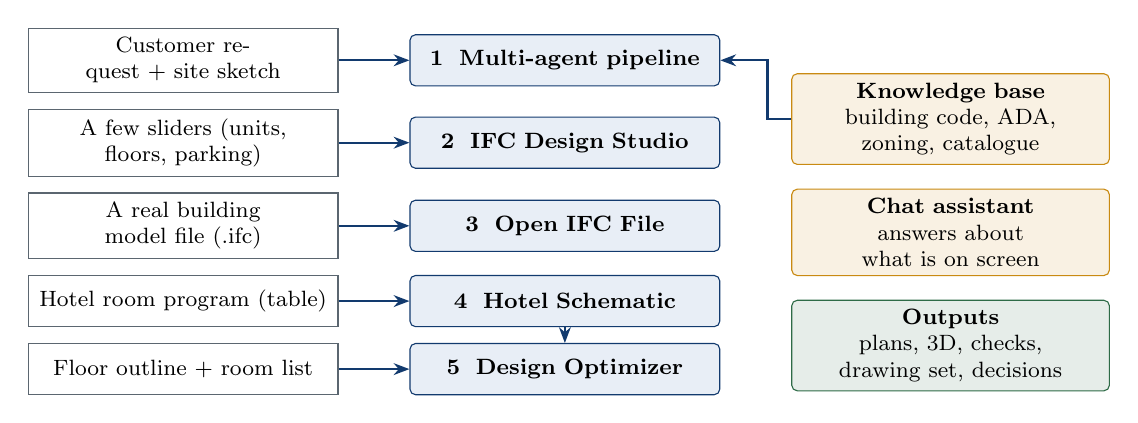
\begin{tikzpicture}[node distance=2mm and 9mm,
  box/.style={draw=blueprintdeep, fill=blueprint!10, rounded corners=2pt, align=center, font=\footnotesize, minimum height=6.5mm, text width=37mm},
  inp/.style={draw=muted, fill=white, align=center, font=\footnotesize, minimum height=6.5mm, text width=37mm},
  side/.style={draw=amber, fill=amber!12, rounded corners=2pt, align=center, font=\footnotesize, text width=38mm, minimum height=9mm},
  arr/.style={-{Stealth[length=2mm]}, thick, blueprintdeep}]
\node[inp] (i1) {Customer request + site sketch};
\node[inp, below=of i1] (i2) {A few sliders (units, floors, parking)};
\node[inp, below=of i2] (i3) {A real building model file (.ifc)};
\node[inp, below=of i3] (i4) {Hotel room program (table)};
\node[inp, below=of i4] (i5) {Floor outline + room list};
\node[box, right=of i1] (m1) {\textbf{1 \ Multi-agent pipeline}};
\node[box, right=of i2] (m2) {\textbf{2 \ IFC Design Studio}};
\node[box, right=of i3] (m3) {\textbf{3 \ Open IFC File}};
\node[box, right=of i4] (m4) {\textbf{4 \ Hotel Schematic}};
\node[box, right=of i5] (m5) {\textbf{5 \ Design Optimizer}};
\node[side, right=of m2, yshift=3mm] (kb) {\textbf{Knowledge base}\\ building code, ADA, zoning, catalogue};
\node[side, below=3mm of kb] (chat) {\textbf{Chat assistant}\\ answers about what is on screen};
\node[side, below=3mm of chat, fill=ok!12, draw=ok] (out) {\textbf{Outputs}\\ plans, 3D, checks, drawing set, decisions};
\foreach \a/\b in {i1/m1,i2/m2,i3/m3,i4/m4,i5/m5} \draw[arr] (\a) -- (\b);
\draw[arr] (kb.west) -- ++(-3mm,0) |- (m1.east);
\draw[arr, dashed] (m4.south) -- (m5.north);
\end{tikzpicture}

\vspace{0.15cm}
{\small One web app with five modes. They share one knowledge base and one chat assistant. The optimizer of Part 1 runs as mode 5 and inside mode 4.}
\end{frame}

% ------------------------------------------------------------------ principle
\begin{frame}{One rule across the whole system}
\centering{\large\color{blueprintdeep}\textbf{The AI model reads and judges. Ordinary code does every calculation.}}
\vspace{0.3cm}
\begin{columns}[T]
\begin{column}{0.31\textwidth}
\begin{block}{Done by code}
Areas, counts, distances, site layout, floor plans, code checks, drawings, the optimizer.

\textbf{Cannot make things up.} Same input, same output.
\end{block}
\end{column}
\begin{column}{0.31\textwidth}
\begin{block}{Done by the AI, with guard rails}
Reading a free-text request, finding limits in code documents, judging conflicts, the final recommendation.

Fixed answer formats, sources cited, ``say unknown rather than guess''.
\end{block}
\end{column}
\begin{column}{0.31\textwidth}
\begin{block}{Free text from the AI}
Explanations, report wording and chat answers.

\textbf{Can be wrong.} These are explanations; the checks computed by code are the facts.
\end{block}
\end{column}
\end{columns}
\vspace{0.3cm}
{\small Why it matters: a wrong number in a building design is expensive. Keeping the arithmetic out of the AI model is what kept invented numbers out of the results.}
\end{frame}

% ------------------------------------------------------------------ pipeline
\begin{frame}{Part 1 of the studio: the multi-agent pipeline}
\begin{columns}[c]
\begin{column}{0.55\textwidth}\centering
\shot{\textwidth}{04_pipeline_agent_trace.png}
\end{column}
\begin{column}{0.41\textwidth}
\textbf{What it does:} takes a customer's written request and a site, and decides whether the project is feasible.

\textbf{How:} a chain of small AI agents, each with one job: read the request, look up the zoning limits, match rooms to BaaP modules, find conflicts, and give a final decision with reasons.

Every step is logged with what it did and how long it took.
\end{column}
\end{columns}
\end{frame}

\begin{frame}{The pipeline: site layout, checking and the decision}
\begin{columns}[c]
\begin{column}{0.48\textwidth}\centering
\shot{0.74\textwidth}{07_pipeline_site_simulation.png}\\[0.1cm]
{\small The building and parking are pushed into place like objects that may not overlap. The finished drawing is then measured again from the image, as an independent check.}
\end{column}
\begin{column}{0.48\textwidth}\centering
\shot{0.74\textwidth}{09_pipeline_final_decision.png}\\[0.1cm]
{\small The final decision, with unresolved issues and next steps.}
\end{column}
\end{columns}
\vspace{0.15cm}
\begin{block}{Result}
Three full runs of the same project all gave the same decision (``revise'', because the surface parking cannot fit). The request was read correctly in 3 of 3 runs and all 9 zoning limits were found in 2 of 2 runs. The wording of the explanation varied between runs.
\end{block}
\end{frame}

% ------------------------------------------------------------------ IFC
\begin{frame}{Parts 2 and 3: building models (IFC)}
\begin{columns}[c]
\begin{column}{0.48\textwidth}\centering
\shot{\textwidth}{10_ifc_baseline_3d_model.png}\\[0.1cm]
{\small \textbf{IFC Design Studio.} Move a few sliders and get a real 3D building model that other design software can open, checked against zoning and RNGD's building-code rules. No AI model is used to create it.}
\end{column}
\begin{column}{0.48\textwidth}\centering
\shot{\textwidth}{17_explorer_3d_model.png}\\[0.1cm]
{\small \textbf{Open IFC File.} Load an existing building model (here a real 89 MB bank building), look at it in 3D, browse its elements and ask questions about it.}
\end{column}
\end{columns}
\end{frame}

% ------------------------------------------------------------------ hotel
\begin{frame}{Part 4: Hotel Schematic}
\begin{columns}[c]
\begin{column}{0.55\textwidth}\centering
\shot{\textwidth}{20_hotel_overview.png}
\end{column}
\begin{column}{0.41\textwidth}
\textbf{What it does:} turns a hotel room program into a complete schematic design.

\textbf{Default input:} RNGD's Living + Lodging program, 117 keys in 28 rows. It can be edited or uploaded.

\textbf{How:} fixed rules, no AI model:
\begin{itemize}
\item guest rooms along a corridor with rooms on both sides
\item public and service rooms on Level 1
\item stairs at both ends, elevators at the core
\end{itemize}
\textbf{Result:} four different programs gave four different, correct buildings, and each rebuild was identical.
\end{column}
\end{columns}
\end{frame}

\begin{frame}{Hotel Schematic: plans, code check and drawings}
\begin{columns}[T]
\begin{column}{0.32\textwidth}\centering
\shot{0.88\textwidth}{24_hotel_plan_level2.png}\\[0.1cm]
{\small Interactive floor plan of a guest floor}
\end{column}
\begin{column}{0.32\textwidth}\centering
\shot{0.88\textwidth}{28_hotel_code.png}\\[0.1cm]
{\small Check against RNGD's building-code rules and the ADA guest-room tables}
\end{column}
\begin{column}{0.32\textwidth}\centering
\shot{0.88\textwidth}{30_hotel_report_sheets.png}\\[0.1cm]
{\small A drawing set in RNGD's sheet format: plans, elevations, unit plans, 3D}
\end{column}
\end{columns}
\vspace{0.3cm}
\begin{block}{A useful catch}
With five guest floors the default program has six levels, one more than the five-story rule in RNGD's rule file allows. The check flags it and suggests four guest floors, which pass.
\end{block}
\end{frame}

% ------------------------------------------------------------------ differences
\begin{frame}{How the five parts differ}
\begingroup\small
\begin{tabular}{@{}p{2.9cm}p{2.9cm}p{3.3cm}p{1.6cm}p{1.6cm}@{}}
\toprule
\textbf{Part} & \textbf{Starts from} & \textbf{Method} & \textbf{AI model?} & \textbf{Repeatable?} \\ \midrule
1 \ Multi-agent pipeline & written request + site & AI agents, document search, site simulation & yes, to read and judge & decision yes, wording no \\
2 \ IFC Design Studio & a few sliders & rules that generate a 3D model & no & yes \\
3 \ Open IFC File & an existing model file & reading and displaying the model & only for chat & yes \\
4 \ Hotel Schematic & a hotel room program & rules for layout, code check and drawings & no & yes \\
5 \ Design Optimizer & floor outline + room list & search over many plans, scored by arithmetic & no (only for report text) & yes \\
\bottomrule
\end{tabular}\par\endgroup
\vspace{0.2cm}
\begin{itemize}
\item Parts 2 and 4 \textbf{build one design} from rules. Part 5 \textbf{searches many designs} and ranks them. Part 1 \textbf{decides} whether a request is feasible.
\item Only part 1 depends on the AI model for its result, and its numbers still come from code.
\end{itemize}
\end{frame}

% ------------------------------------------------------------------ results
\begin{frame}{Results in one slide}
\begin{columns}[T]
\begin{column}{0.47\textwidth}
\begin{block}{Layout optimization}
\begin{itemize}
\item 171 $\rightarrow$ 197 rooms placed over three sites
\item 24 $\rightarrow$ 0 guest rooms without a window
\item All code checks pass on every site
\item About 20 seconds per site, repeatable
\item 740 hotel layouts with generated shapes in about 36 seconds
\end{itemize}
\end{block}
\begin{block}{Quality}
All 51 automated tests pass, including tests that drive the real app.
\end{block}
\end{column}
\begin{column}{0.47\textwidth}
\begin{block}{The rest of the studio}
\begin{itemize}
\item Pipeline: same decision in 3 of 3 runs; every number in its explanation traced back to computed data
\item Hotel generator: four programs, four correct buildings, identical on rebuild
\item A complete drawing set in RNGD's sheet format, generated from the program
\item RNGD's real building-code rules and the ADA standard are used for the checks
\end{itemize}
\end{block}
\end{column}
\end{columns}
\end{frame}

% ------------------------------------------------------------------ limits
\begin{frame}{What is still open, and next steps}
\begin{columns}[T]
\begin{column}{0.47\textwidth}
\begin{block}{Honest limits}
\begin{itemize}
\item The optimized hotel layout places all 117 keys but leaves out 8 of 150 rooms (retail, gym and some service rooms): the ground floor uses the same outline as the guest floors
\item The reference optimizer's run time was not recorded, so I cannot compare speed with it
\item Optimized layouts are shown as plans and 3D, not yet as drawing sheets
\item Pipeline inputs and the BaaP catalogue are sample data
\item No parking, structure or MEP yet
\end{itemize}
\end{block}
\end{column}
\begin{column}{0.47\textwidth}
\begin{block}{Next steps}
\begin{itemize}
\item A wider ground floor (podium) so all public rooms fit
\item Drawing sheets straight from the optimized layouts
\item RNGD's real module and panel catalogue
\item More of the building-code rule set
\item Parking and structural grid
\end{itemize}
\end{block}
\begin{block}{Questions for RNGD}
Is a podium intended, as in the Living + Lodging prototype? Which module and panel sizes should the bays follow?
\end{block}
\end{column}
\end{columns}
\end{frame}

% ------------------------------------------------------------------ close
{\setbeamertemplate{footline}{}
\begin{frame}[plain]
\begin{tikzpicture}[remember picture,overlay]
  \fill[blueprintdeep] (current page.south west) rectangle (current page.north east);
\end{tikzpicture}
\vspace*{1.2cm}
{\color{paper}\fontsize{26}{30}\selectfont\bfseries Thank you}\\[0.6cm]
{\color{paper!85}\large In one sentence: once the optimizer can only build plans that make architectural sense,\\ a simple, repeatable search places more rooms and gives every guest room a window.}\\[1.0cm]
{\color{amber}\large Questions?}\\[0.9cm]
{\color{paper!65}\small Details: walkthrough report, the paper, and the optimization-algorithms report in \texttt{reports/}}
\end{frame}}

\end{document}
